% Section 5: Experiment 2 — Expanded Library (v3) (~2.5 pages)

\subsection{Design Rationale}

Experiment~1 diagnosed three design flaws that prevented weight learning from improving retrieval:
(a)~too few skills (50), causing a small number of generic meta-skills to dominate;
(b)~skills too domain-general, making all skills roughly equally relevant to any task;
(c)~recency and importance dimensions near-saturated (${\sim}$0.95), leaving only relevance with meaningful variance.
Experiment~1 also used \texttt{max\_tokens}$=$4{,}096, which introduced truncation cascades: every non-final step hit the output limit, causing the runner to continue iterating with accumulated context.
This confound inflated multi-step rates and made it impossible to distinguish genuine behavioral effects from truncation artifacts.

Experiment~2 addresses all four issues:
\begin{itemize}
\item \textbf{205 domain-specific skills:} 30 base skills plus 175 specialized skills (${\sim}$35 per theme), ensuring that topic-specific tasks have enough candidate skills for weight differences to change rankings.
\item \textbf{12 weight presets:} The original 5 plus 7 new presets including extreme configurations (85/5/10) and an anti-relevance preset (45/45/10) that explicitly tests whether de-emphasizing semantic similarity helps for certain task types.
\item \textbf{300 harder tasks:} 50 easy, 100 medium, 150 hard, shifting the distribution toward tasks where retrieval quality should matter most.
\item \textbf{\texttt{max\_tokens}$=$16{,}384:} Eliminates truncation cascades by ensuring the LLM can always complete its response in a single generation.
\end{itemize}

\paragraph{Key predictions.}
If the fix works: (1)~Jaccard overlap between conditions should drop from $>$0.90 to $<$0.60; (2)~bandit convergence in C2/C3 should correlate with improved ground truth hit rate; (3)~C4 should either develop convergence (if the anchor parser produces enough variance with 12 arms) or remain the ``rubric-only'' baseline.

\subsection{Results}

\begin{table}[t]
\centering
\small
\begin{tabular}{lrrrrrr}
\toprule
\textbf{Cond.} & \textbf{Mean Tok.} & \textbf{Med.} & \textbf{SD} & \textbf{$\Delta$C1} & \textbf{NDCG@5} & \textbf{Jacc.} \\
\midrule
C1 & 5{,}517 & 4{,}910 & 2{,}449 & --- & 0.371 & --- \\
C2 & 4{,}824 & 4{,}204 & 1{,}896 & $-$12.6\% & 0.394 & 0.585 \\
C3 & 4{,}830 & 4{,}286 & 1{,}820 & $-$12.5\% & 0.469 & 0.517 \\
C4 & 4{,}429 & 4{,}100 & 1{,}429 & $-$19.7\% & 0.374 & 0.573 \\
\bottomrule
\end{tabular}
\caption{Experiment~2 main results ($N{=}300$ per condition, 1{,}200 total episodes). Token reduction is relative to C1 mean. Jaccard reports mean per-episode overlap of top-5 retrieved skill sets against C1. Only 1 of 1{,}200 episodes triggered multi-step reasoning. Kruskal--Wallis $H(3){=}33.87$, $p{<}0.001$. All three C1-vs-treatment comparisons survive Holm--Bonferroni correction ($p{<}0.001$).}
\label{tab:v3_results}
\end{table}

\paragraph{Token efficiency.}
Table~\ref{tab:v3_results} summarizes the main results.
All three feedback conditions reduce mean token consumption by 12--20\% relative to C1, with C4 achieving the largest reduction ($-$19.7\%).
The Kruskal--Wallis test confirms that the four conditions differ significantly ($H(3){=}33.87$, $p{<}0.001$).
After Holm--Bonferroni correction for six pairwise comparisons, all three C1-vs-treatment comparisons remain significant: C1 vs.\ C4 ($p{<}0.001$, $d{=}0.543$), C1 vs.\ C2 ($p{=}0.0003$, $d{=}0.317$), and C1 vs.\ C3 ($p{=}0.0004$, $d{=}0.319$).
Treatment-vs-treatment comparisons are not significant after correction.
BCa bootstrap 95\% CIs for the mean difference (10{,}000 resamples) are C1$-$C2: $[340,\, 1{,}052]$, C1$-$C3: $[341,\, 1{,}033]$, C1$-$C4: $[772,\, 1{,}418]$; all exclude zero (Figure~\ref{fig:v3_token_boxplot}).

\begin{figure}[t]
\centering
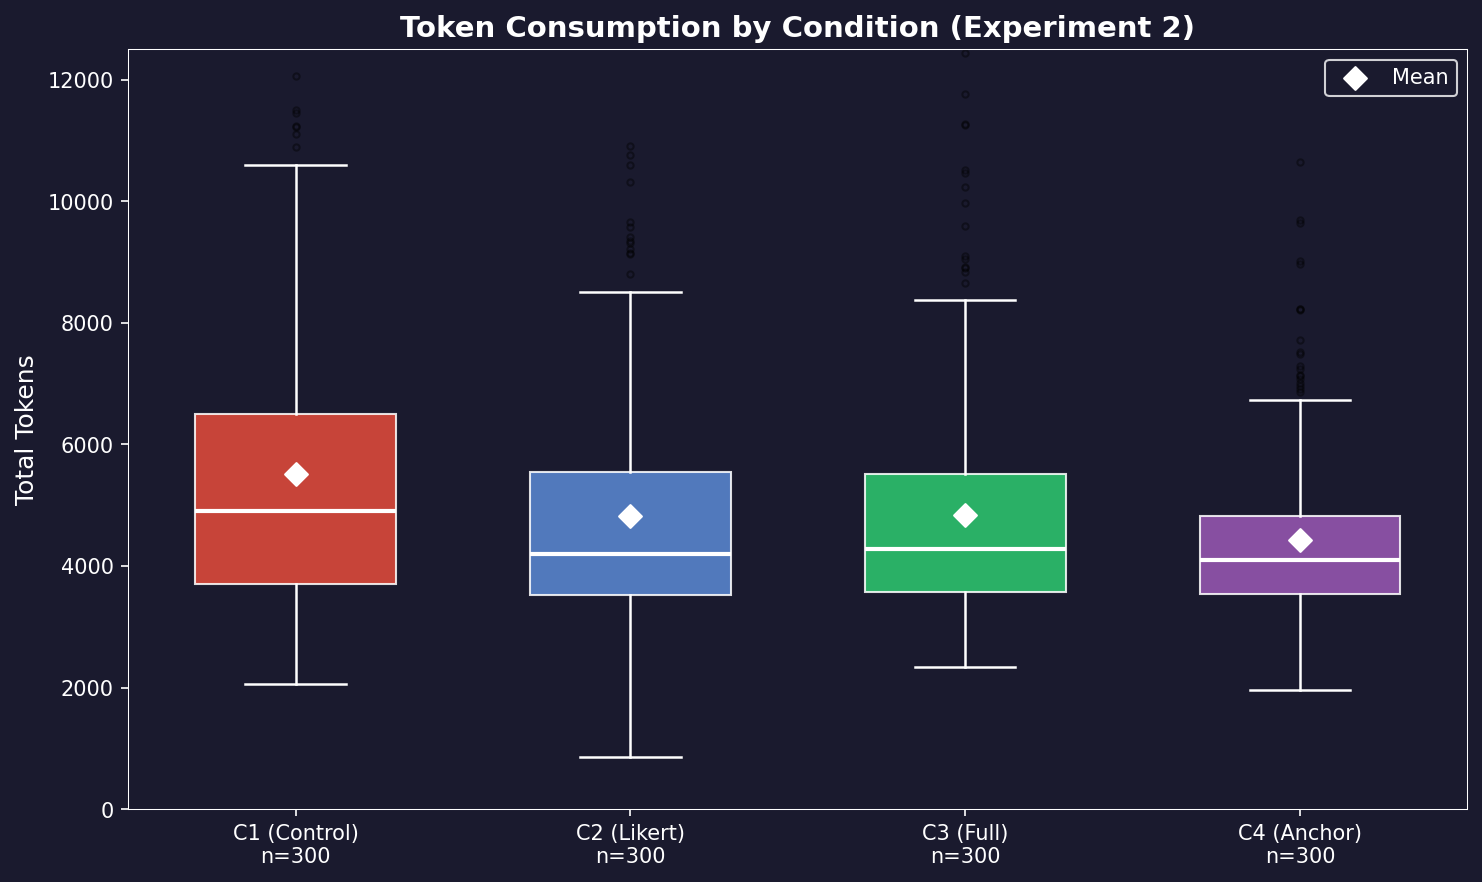
\includegraphics[width=\columnwidth]{../results/figures/fig1_v3_token_boxplot.png}
\caption{Token consumption distributions by condition (v3). With truncation cascades eliminated (\texttt{max\_tokens}$=$16{,}384), all conditions produce unimodal distributions with moderate right skew. The treatment effect is visible as a shift in both location and spread: C4 SD${=}$1{,}429 vs.\ C1 SD${=}$2{,}449.}
\label{fig:v3_token_boxplot}
\end{figure}

\paragraph{Output-driven mechanism.}
Unlike Experiment~1, where the treatment effect was driven by multi-step prevention (a truncation artifact), Experiment~2 reveals the underlying mechanism: feedback conditions produce \emph{shorter LLM outputs}.
Only 1 of 1{,}200 episodes triggered multi-step reasoning (C1, task~023, 2 steps, 21{,}259 tokens), effectively eliminating multi-step behavior as an explanatory variable.
Instead, the token reduction is concentrated in output tokens: C1 generates a mean of 3{,}813 output tokens per episode, compared to 2{,}960 (C2, $-$22\%), 2{,}946 (C3, $-$23\%), and 2{,}537 (C4, $-$33\%).
Input tokens are comparable across conditions (${\sim}$1{,}700--1{,}890), confirming that the difference lies in generation length, not prompt construction.

This suggests two separable effects: improved retrieval quality from weight learning, and the structured rubric prompt producing more focused output.
The rubric's metacognitive scaffolding appears to reduce verbose exploration in the LLM's output independently of which skills were retrieved, an effect that operates through prompt structure rather than retrieval architecture.

\paragraph{Input/output token split.}
C1 episodes are 69\% output tokens (0.45:1 input-to-output ratio), while feedback conditions shift toward higher input proportions: C2 61\% output (0.63:1), C3 61\% (0.64:1), C4 57\% (0.75:1).
The increasing input-to-output ratio from C1 to C4 is consistent with the rubric adding structured input tokens while the LLM produces proportionally shorter outputs (Figure~\ref{fig:v3_io_tokens}).

\begin{figure}[t]
\centering
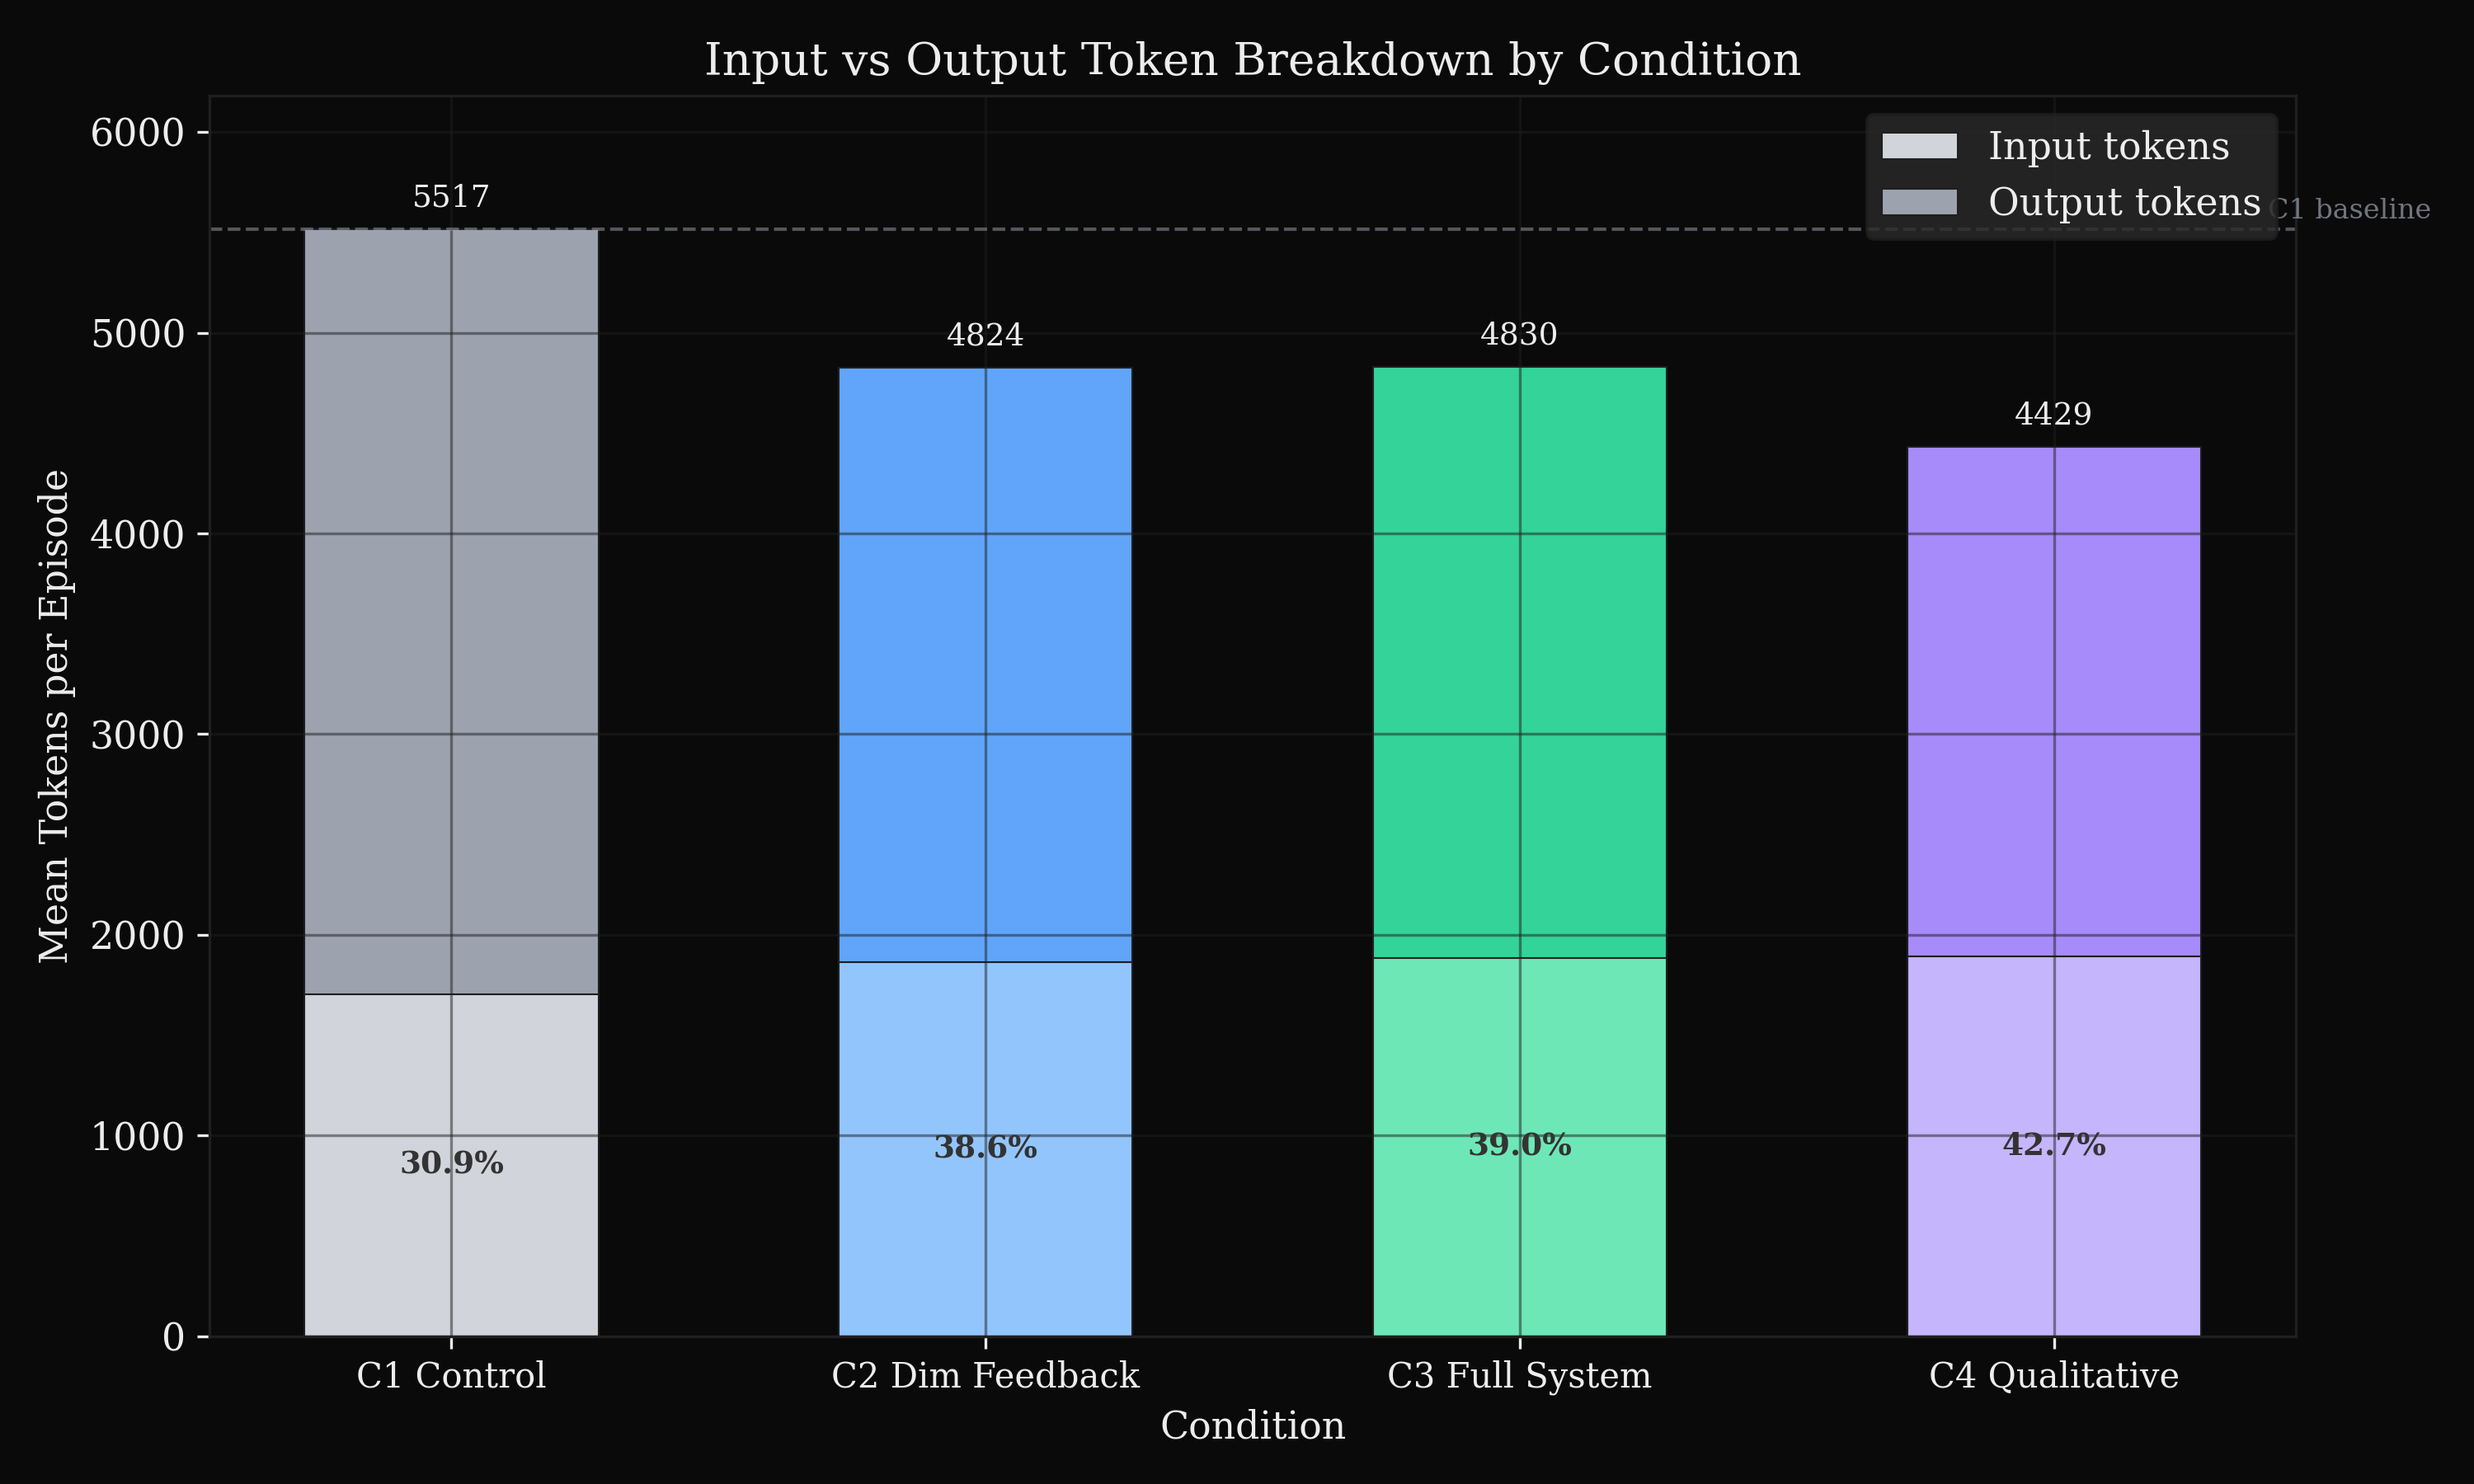
\includegraphics[width=\columnwidth]{../results/figures/figIO1_stacked_bar_tokens.png}
\caption{Input vs.\ output token breakdown by condition (v3). The treatment effect is concentrated in output tokens: C4 produces 33\% fewer output tokens than C1, while input tokens are comparable across conditions (${\sim}$1{,}700--1{,}890). The increasing input-to-output ratio from C1 (0.45:1) to C4 (0.75:1) reflects the rubric adding structured input while the LLM generates proportionally shorter outputs.}
\label{fig:v3_io_tokens}
\end{figure}

\paragraph{Temporal trend.}
C1 shows stable token consumption across the experiment (first half: 5{,}564, second half: 5{,}471, $-$1.7\%).
C2 shows a modest learning effect: 5{,}055$\,\rightarrow\,$4{,}594 ($-$9.1\%), consistent with the bandit gradually improving its weight selection.
C3 ($-$1.9\%) and C4 ($+$0.8\%) are essentially stable, suggesting that C3's retrieval quality improvements do not translate into further token savings once the rubric effect is accounted for, and C4's anchor-based feedback does not produce a detectable learning trajectory on this metric.

\subsection{Retrieval Differentiation}

The central question of Experiment~2 is whether the expanded library and de-saturated dimensions enable weight learning to genuinely change retrieved skills.

\paragraph{Jaccard overlap.}

\begin{figure}[t]
\centering
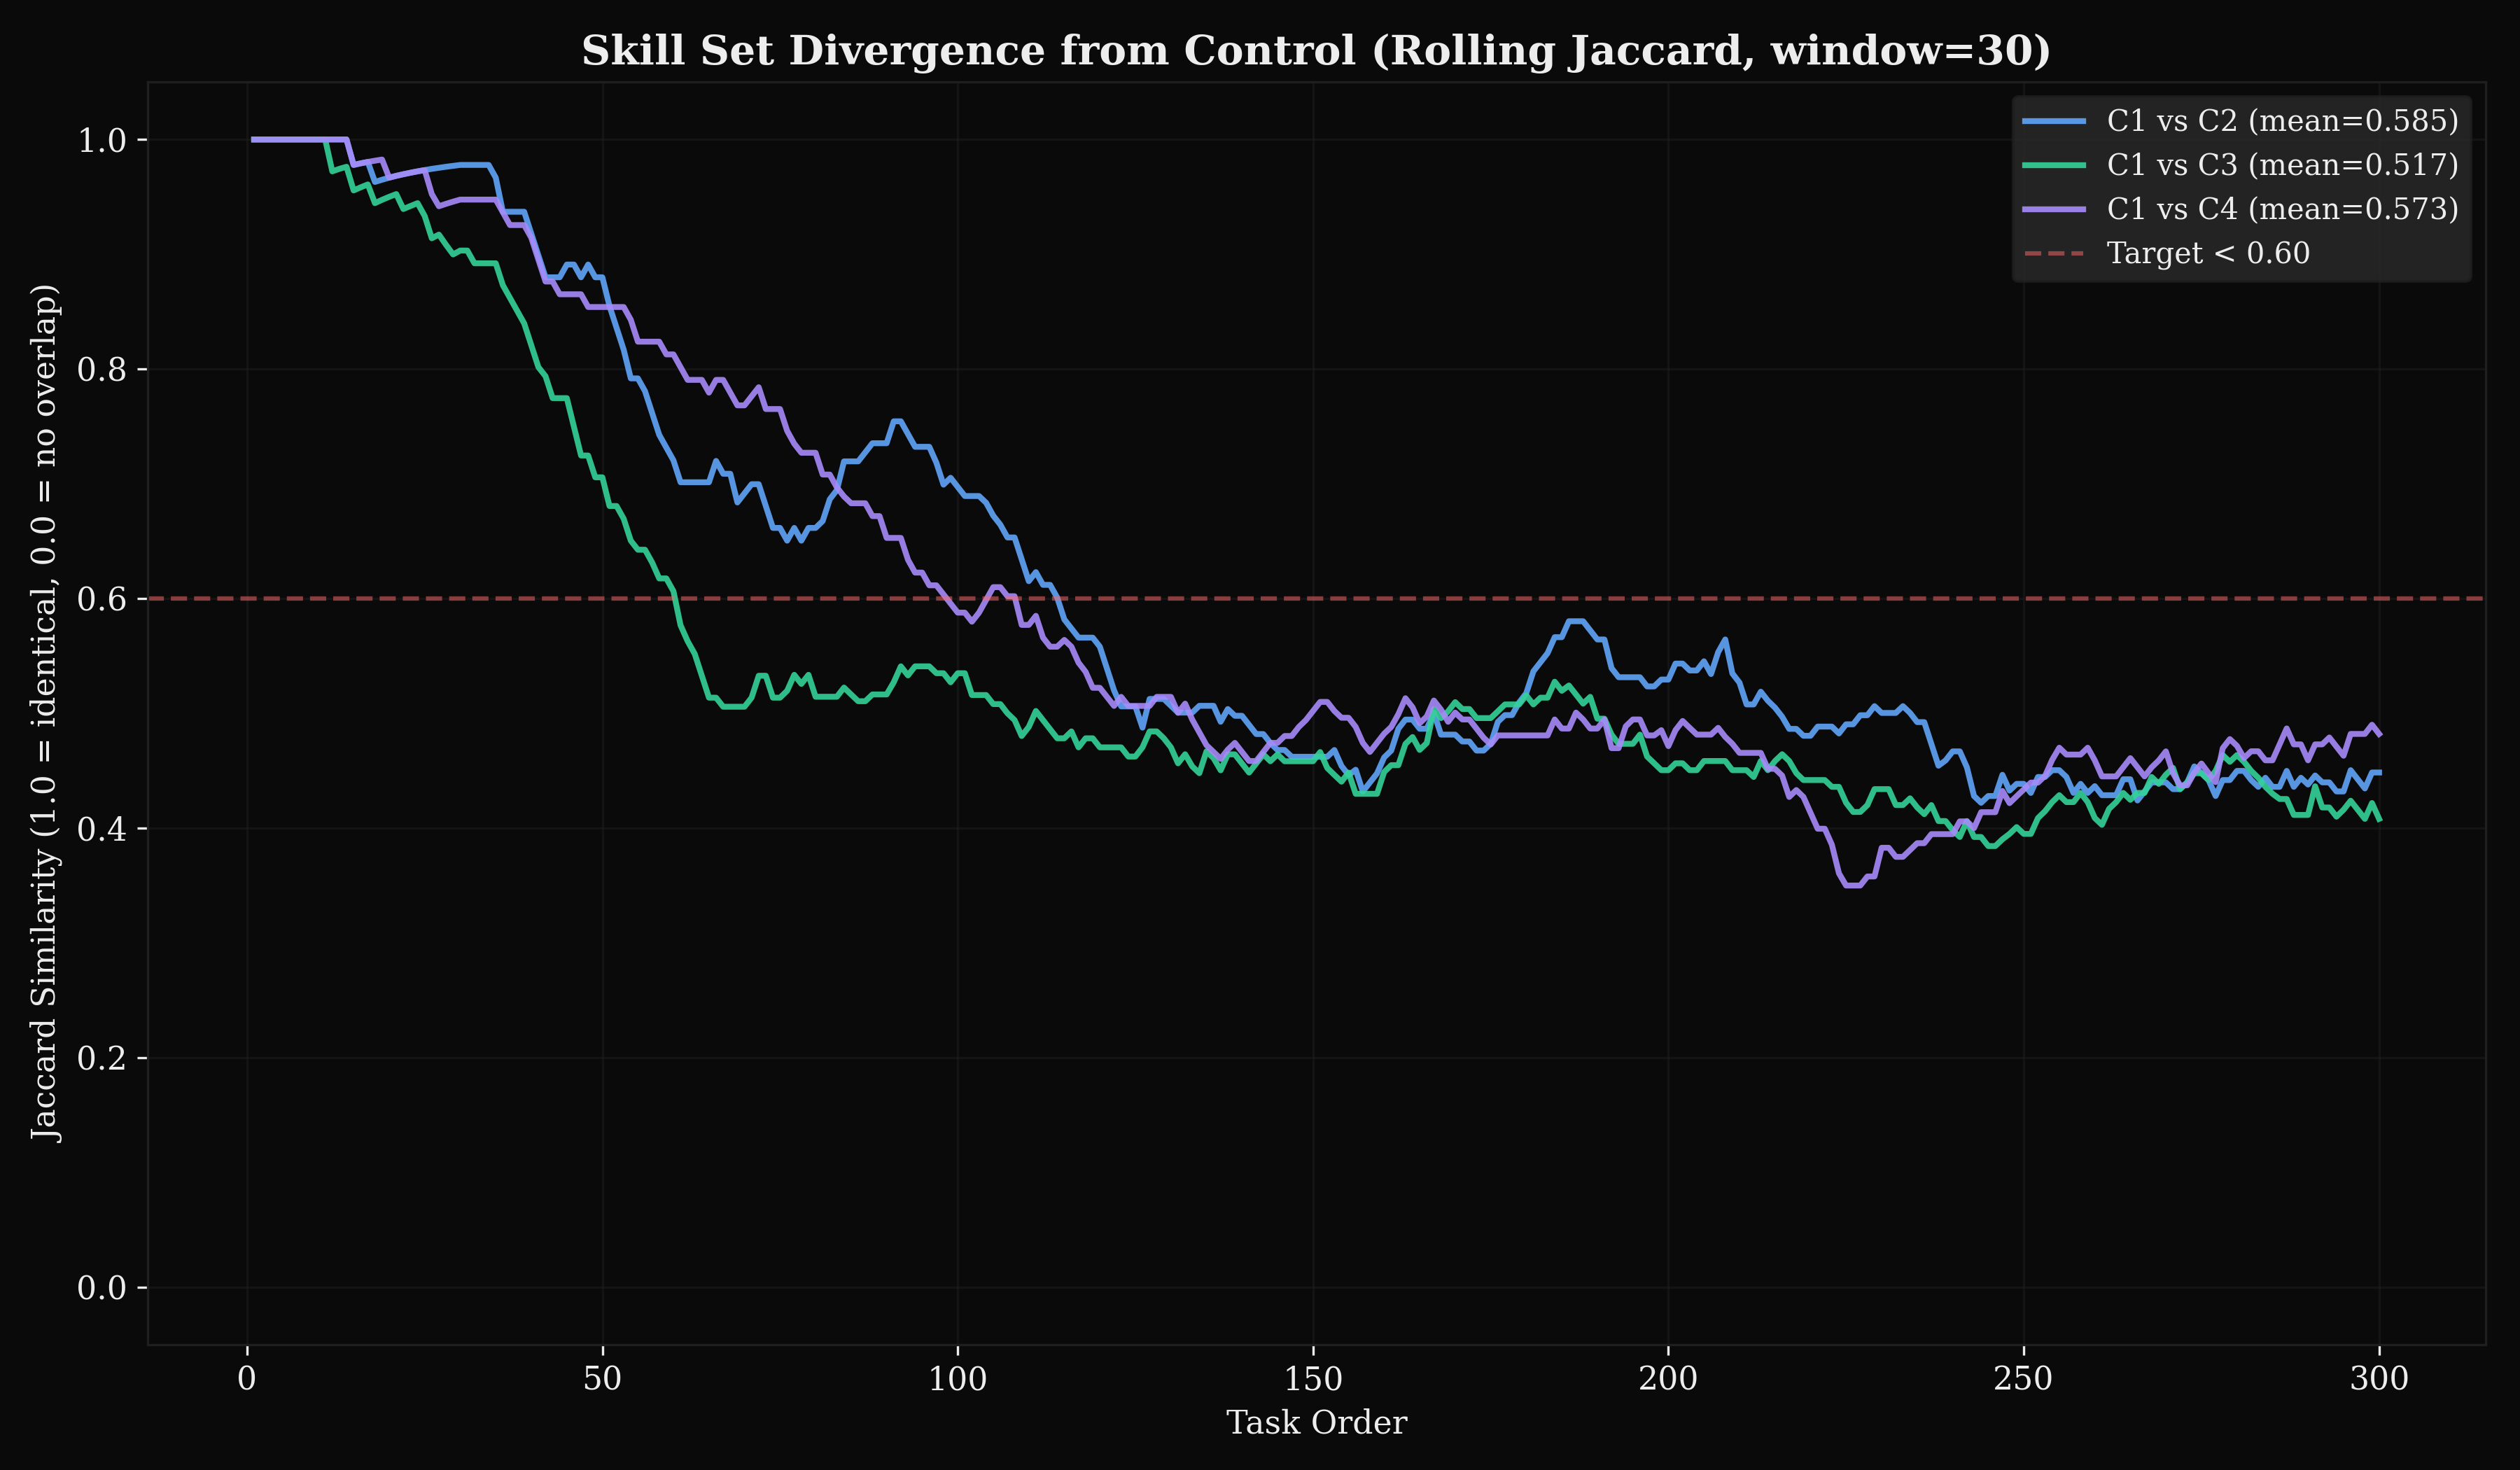
\includegraphics[width=\columnwidth]{../results/figures/fig7_jaccard_trajectory.png}
\caption{Pairwise Jaccard similarity of top-5 retrieved skills over episodes. In v2, all C1-vs-treatment pairs were above 0.84, indicating near-identical retrievals regardless of weight configuration. In v3, C1-vs-treatment pairs drop to 0.52--0.59, meeting the \emph{a priori} $<$0.60 threshold and confirming that weight learning now produces meaningfully different skill sets.}
\label{fig:v3_jaccard_trajectory}
\end{figure}

Mean per-episode Jaccard drops from $>$0.90 (v2) to 0.585 (C1 vs.\ C2), 0.517 (C1 vs.\ C3), and 0.573 (C1 vs.\ C4).
All three C1-vs-treatment values are at or below the 0.60 threshold set \emph{a priori}, confirming that different weight configurations now retrieve meaningfully different skill sets (Table~\ref{tab:v3_results}, Figure~\ref{fig:v3_jaccard_trajectory}).
C3 achieves the lowest overlap with C1 (0.517), consistent with its stronger bandit convergence driving more distinctive weight selections.
The reduction from v2 (0.90$\,\rightarrow\,$0.52--0.59) represents a ${\sim}$37\% decrease in retrieval overlap.

\paragraph{Unique skill usage.}
All conditions use the expanded library broadly: C1 uses 158 unique skills, C2 uses 169, C3 uses 163, and C4 uses 151.
Unlike v2, where C1 was restricted to 5 generic meta-skills, the expanded library ensures that even the control condition accesses diverse skills.
The differentiation between conditions is therefore not in \emph{which} skills are accessible, but in \emph{how they are ranked}, precisely the mechanism that weight learning targets.

\paragraph{Ground truth hit rate.}
Each task has 1--3 annotated ground truth skills.
C1 achieves a 59.7\% hit rate (at least one ground truth skill in the top-5), compared to 59.3\% for C2, 67.3\% for C3, and 58.0\% for C4 (Figure~\ref{fig:v3_gt_hit_rate}).
The rank-aware retrieval metrics show a clearer separation: NDCG@5 is 0.371 (C1), 0.394 (C2), 0.469 (C3), 0.374 (C4); MRR is 0.302 (C1), 0.331 (C2), 0.411 (C3), 0.313 (C4).
C3 achieves the best retrieval quality across all metrics, with NDCG@5 $+$26.3\% and MRR $+$35.9\% relative to C1 (descriptive comparisons; formal significance tests were not conducted for rank-aware retrieval metrics).
This suggests that the explanation embedding pipeline produces a higher-quality reward signal that enables more effective weight learning.

\begin{figure}[t]
\centering
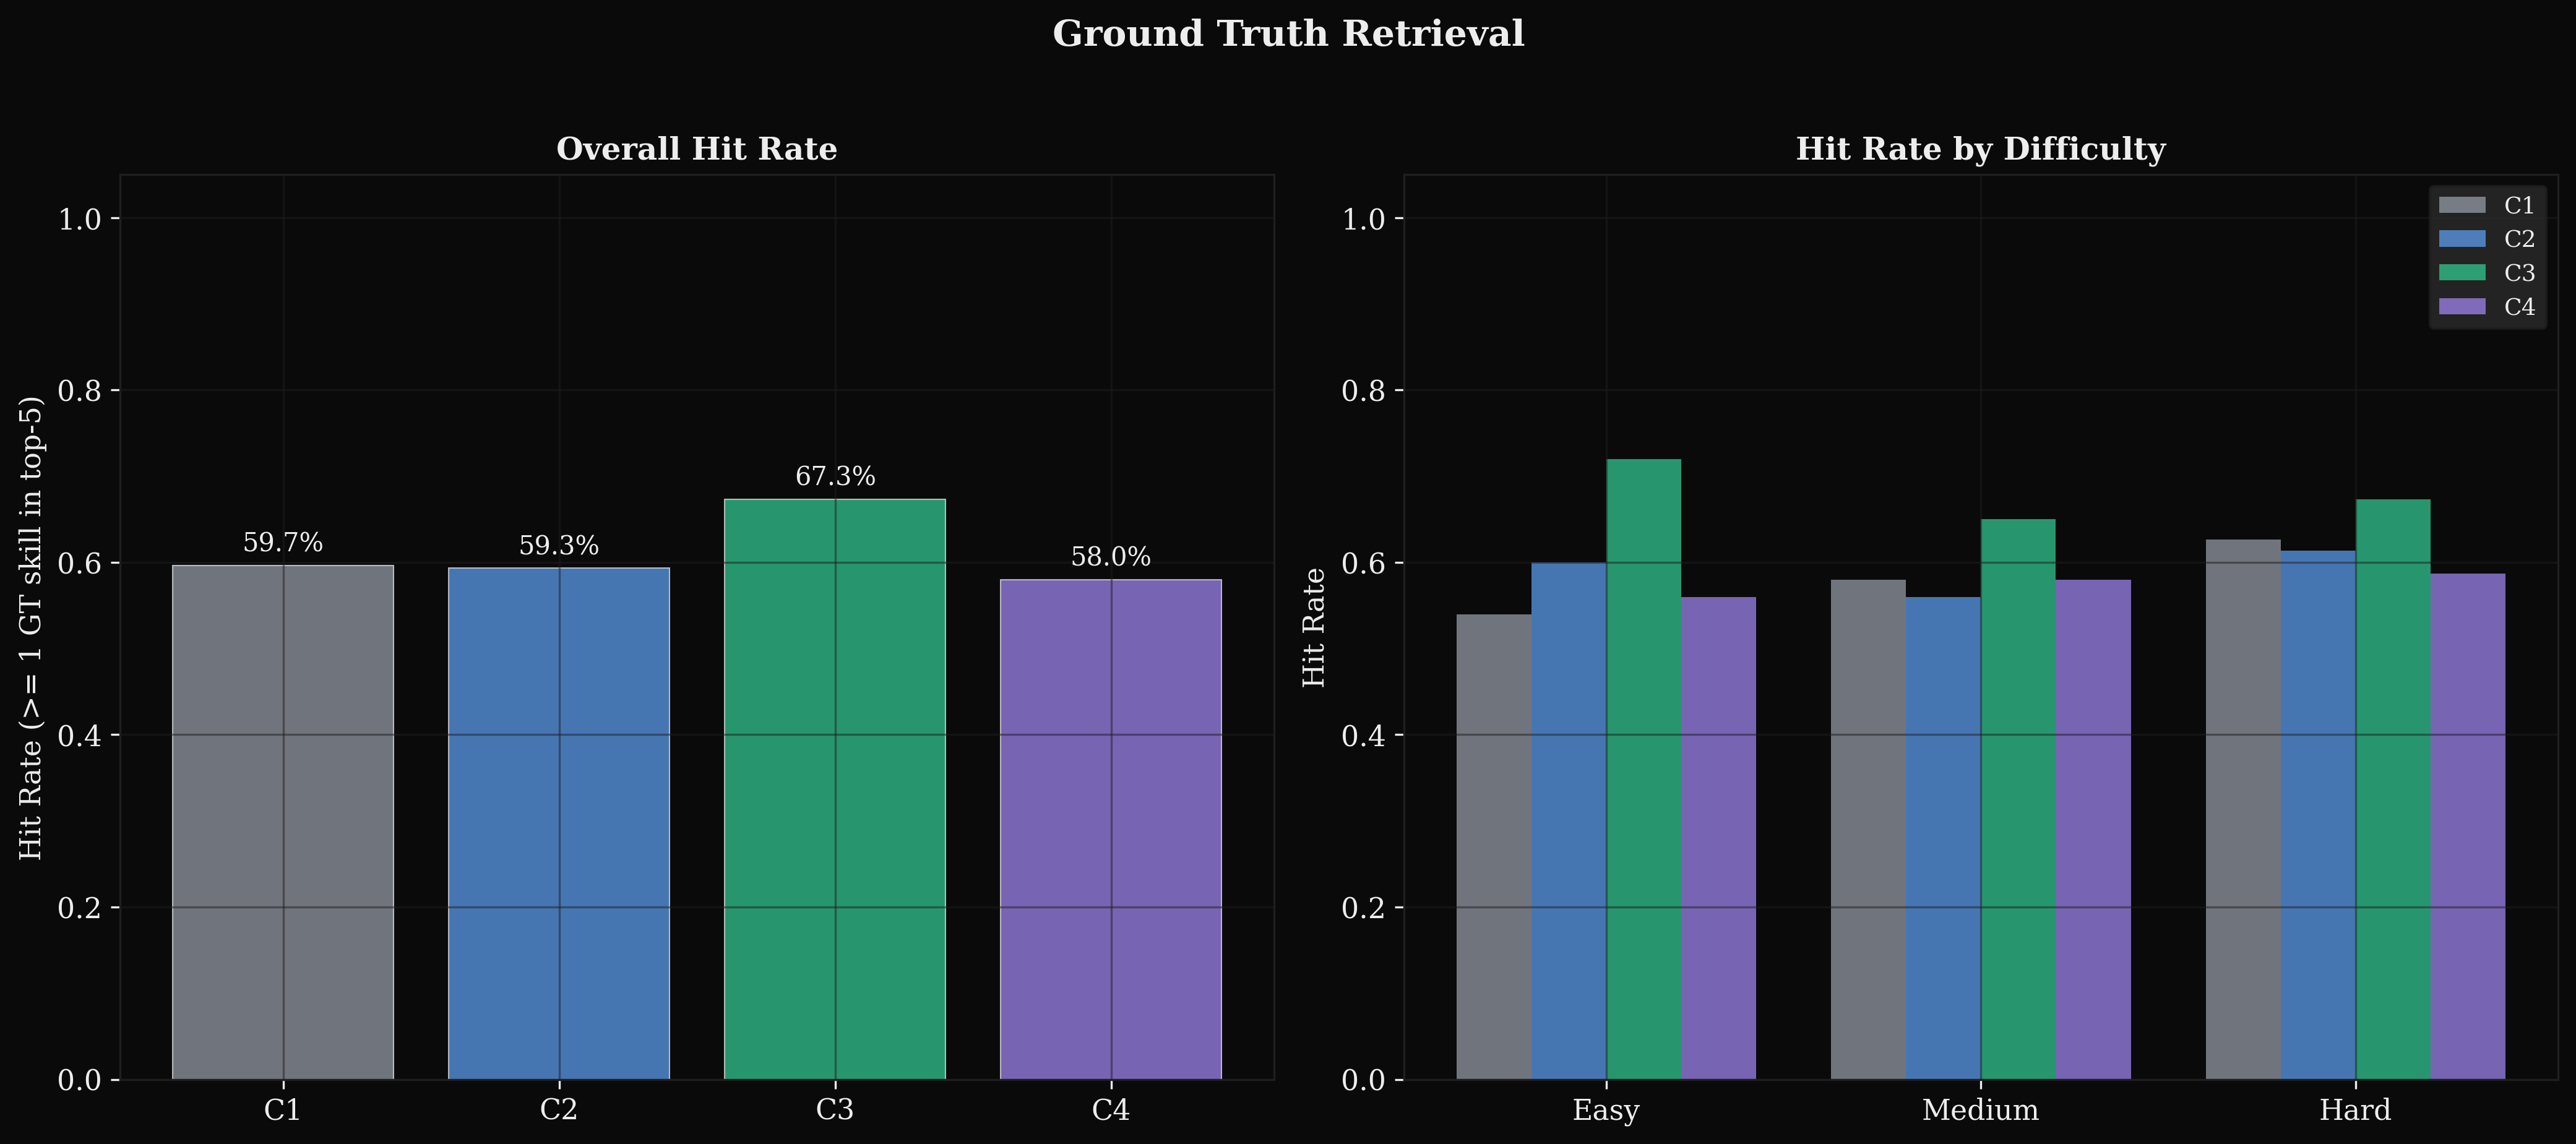
\includegraphics[width=\columnwidth]{../results/figures/fig6_ground_truth_hit_rate.png}
\caption{Retrieval quality by condition (v3). C3 (Full System) achieves the highest NDCG@5 and MRR, consistent with explanation embeddings producing a higher-fidelity reward signal for Thompson Sampling. The improvement is concentrated in ranking quality (NDCG, MRR) rather than binary hit rate, suggesting that weight learning improves skill \emph{ordering} more than skill \emph{selection}.}
\label{fig:v3_gt_hit_rate}
\end{figure}

\subsection{Bandit Convergence}
\label{sec:v3_convergence}

With 12 arms and 300 episodes, Thompson Sampling exhibits three qualitatively distinct convergence patterns (Figure~\ref{fig:v3_bandit_posteriors}).

\textbf{C2 (Likert feedback)} converges to \texttt{pure\_relevance} ($E[\theta]{=}0.709$, 41 pulls), with \texttt{recency\_heavy} as the second-most-pulled arm (50 pulls, $E[\theta]{=}0.704$).
This is a notable shift from Experiment~1, where C2 converged to the importance-heavy preset.
With de-saturated dimensions and specialized skills, the Likert reward signal correctly identifies that semantic relevance is the most informative dimension for retrieval in this library.

\textbf{C3 (Full System)} converges more decisively to \texttt{pure\_relevance} ($E[\theta]{=}0.749$, 73 pulls), with the widest gap over the second arm (\texttt{relevance\_heavy}, $E[\theta]{=}0.719$).
C3's stronger convergence, both higher posterior mean and more concentrated pulls, suggests that the explanation embedding pipeline produces a higher signal-to-noise reward than C2's Likert scores.
The bandit reaches a stable selection pattern by approximately task 33--48, after which \texttt{pure\_relevance} dominates the selection distribution.

\textbf{C4 (Qualitative anchors)} converges weakly to \texttt{pure\_importance} ($E[\theta]{=}0.472$, 35 pulls), with the remaining arms clustered between 0.440 and 0.455.
Unlike the v2 finding of completely flat posteriors, C4 does exhibit a preference, but the compressed posterior range (0.440--0.472) indicates that the anchor parser's reward signal has insufficient variance to drive strong differentiation.

\begin{figure}[t]
\centering
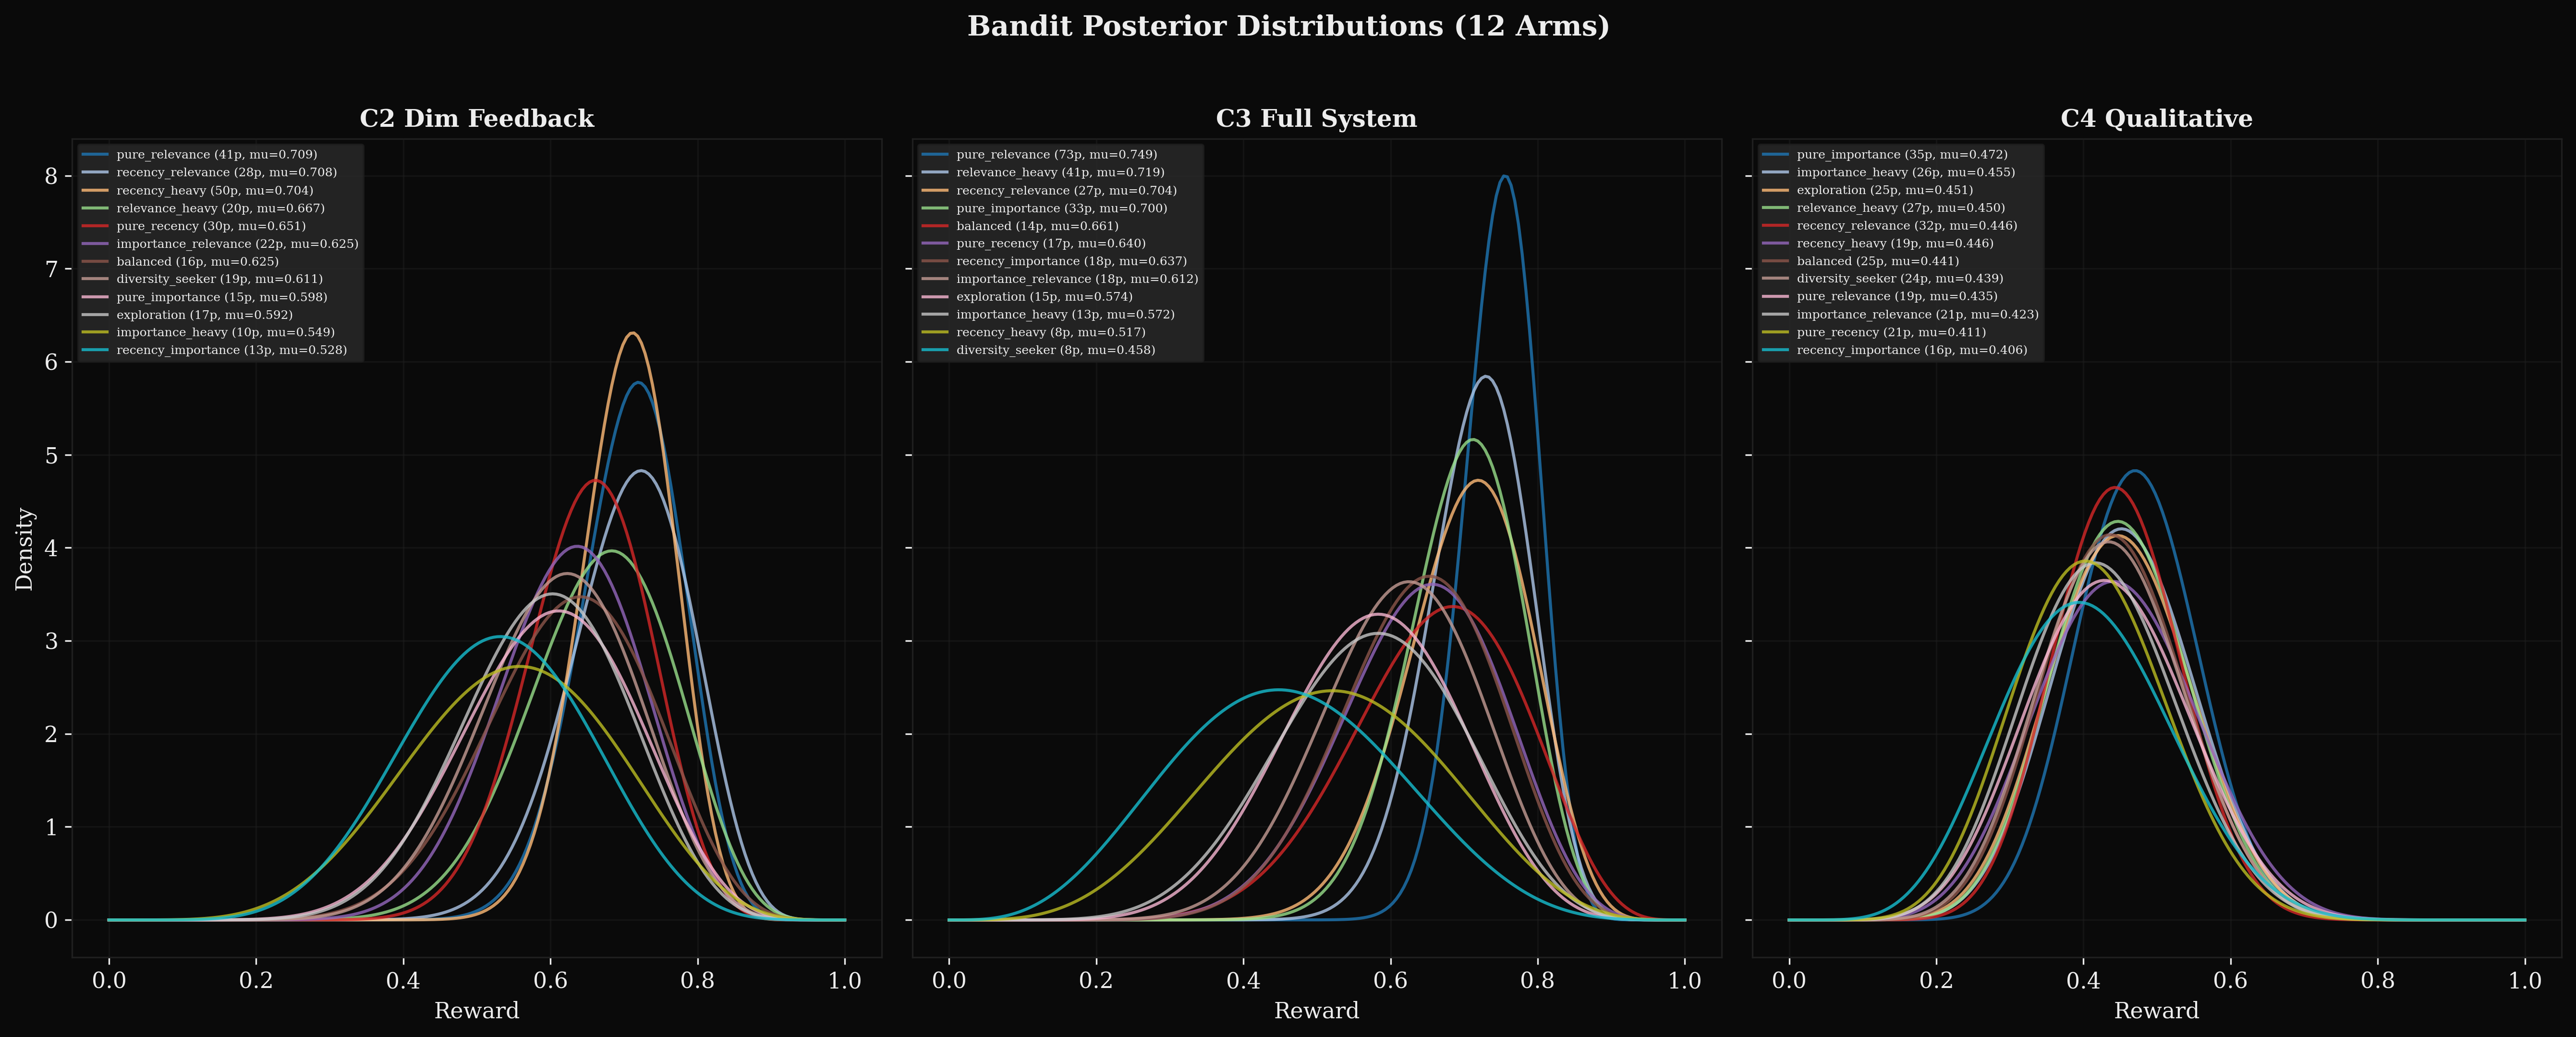
\includegraphics[width=\columnwidth]{../results/figures/figA7_bandit_posteriors.png}
\caption{Thompson Sampling posterior means over episodes (v3, 12 arms). C2 and C3 converge to \texttt{pure\_relevance}, confirming that semantic relevance is the most informative retrieval dimension when the skill library provides sufficient diversity. C4 converges weakly to \texttt{pure\_importance}, with compressed posteriors reflecting the anchor parser's limited discriminative signal.}
\label{fig:v3_bandit_posteriors}
\end{figure}

\paragraph{C4 anchor spread.}
The C4 anchor parser produces per-dimension scores of recency mean${=}$0.14 (SD${=}$0.07), importance mean${=}$0.62 (SD${=}$0.17), relevance mean${=}$0.55 (SD${=}$0.13).
The recency dimension is effectively dead: the ``high recency'' anchor text describes an extreme that typical LLM responses rarely approach, causing the softmax projection to consistently assign low recency scores.
This compressed recency signal explains C4's convergence to \texttt{pure\_importance} rather than \texttt{pure\_relevance}: the bandit optimizes over the dimensions with usable variance.
Parse rates are high across conditions (C2: 93.7\%, C3: 95.0\%, C4: 96.7\%), confirming that C4's weaker convergence is a signal fidelity issue, not a parsing failure.

\subsection{Analysis}

\paragraph{Per-difficulty breakdown.}
The output-driven efficiency effect scales with task difficulty.
Easy tasks: C1${=}$3{,}995, C4${=}$3{,}523 ($-$12\%).
Medium tasks: C1${=}$5{,}573, C4${=}$4{,}409 ($-$21\%).
Hard tasks: C1${=}$5{,}987, C4${=}$4{,}745 ($-$21\%).
All difficulty levels show reductions, but the effect is larger for medium and hard tasks, where C1 generates longer outputs (mean output: easy${=}$2{,}295, medium${=}$3{,}883, hard${=}$4{,}273).
The rubric's metacognitive scaffolding appears most effective when the LLM faces complex tasks that would otherwise produce verbose, exploratory responses (Figure~\ref{fig:v3_difficulty}).

\begin{figure}[t]
\centering
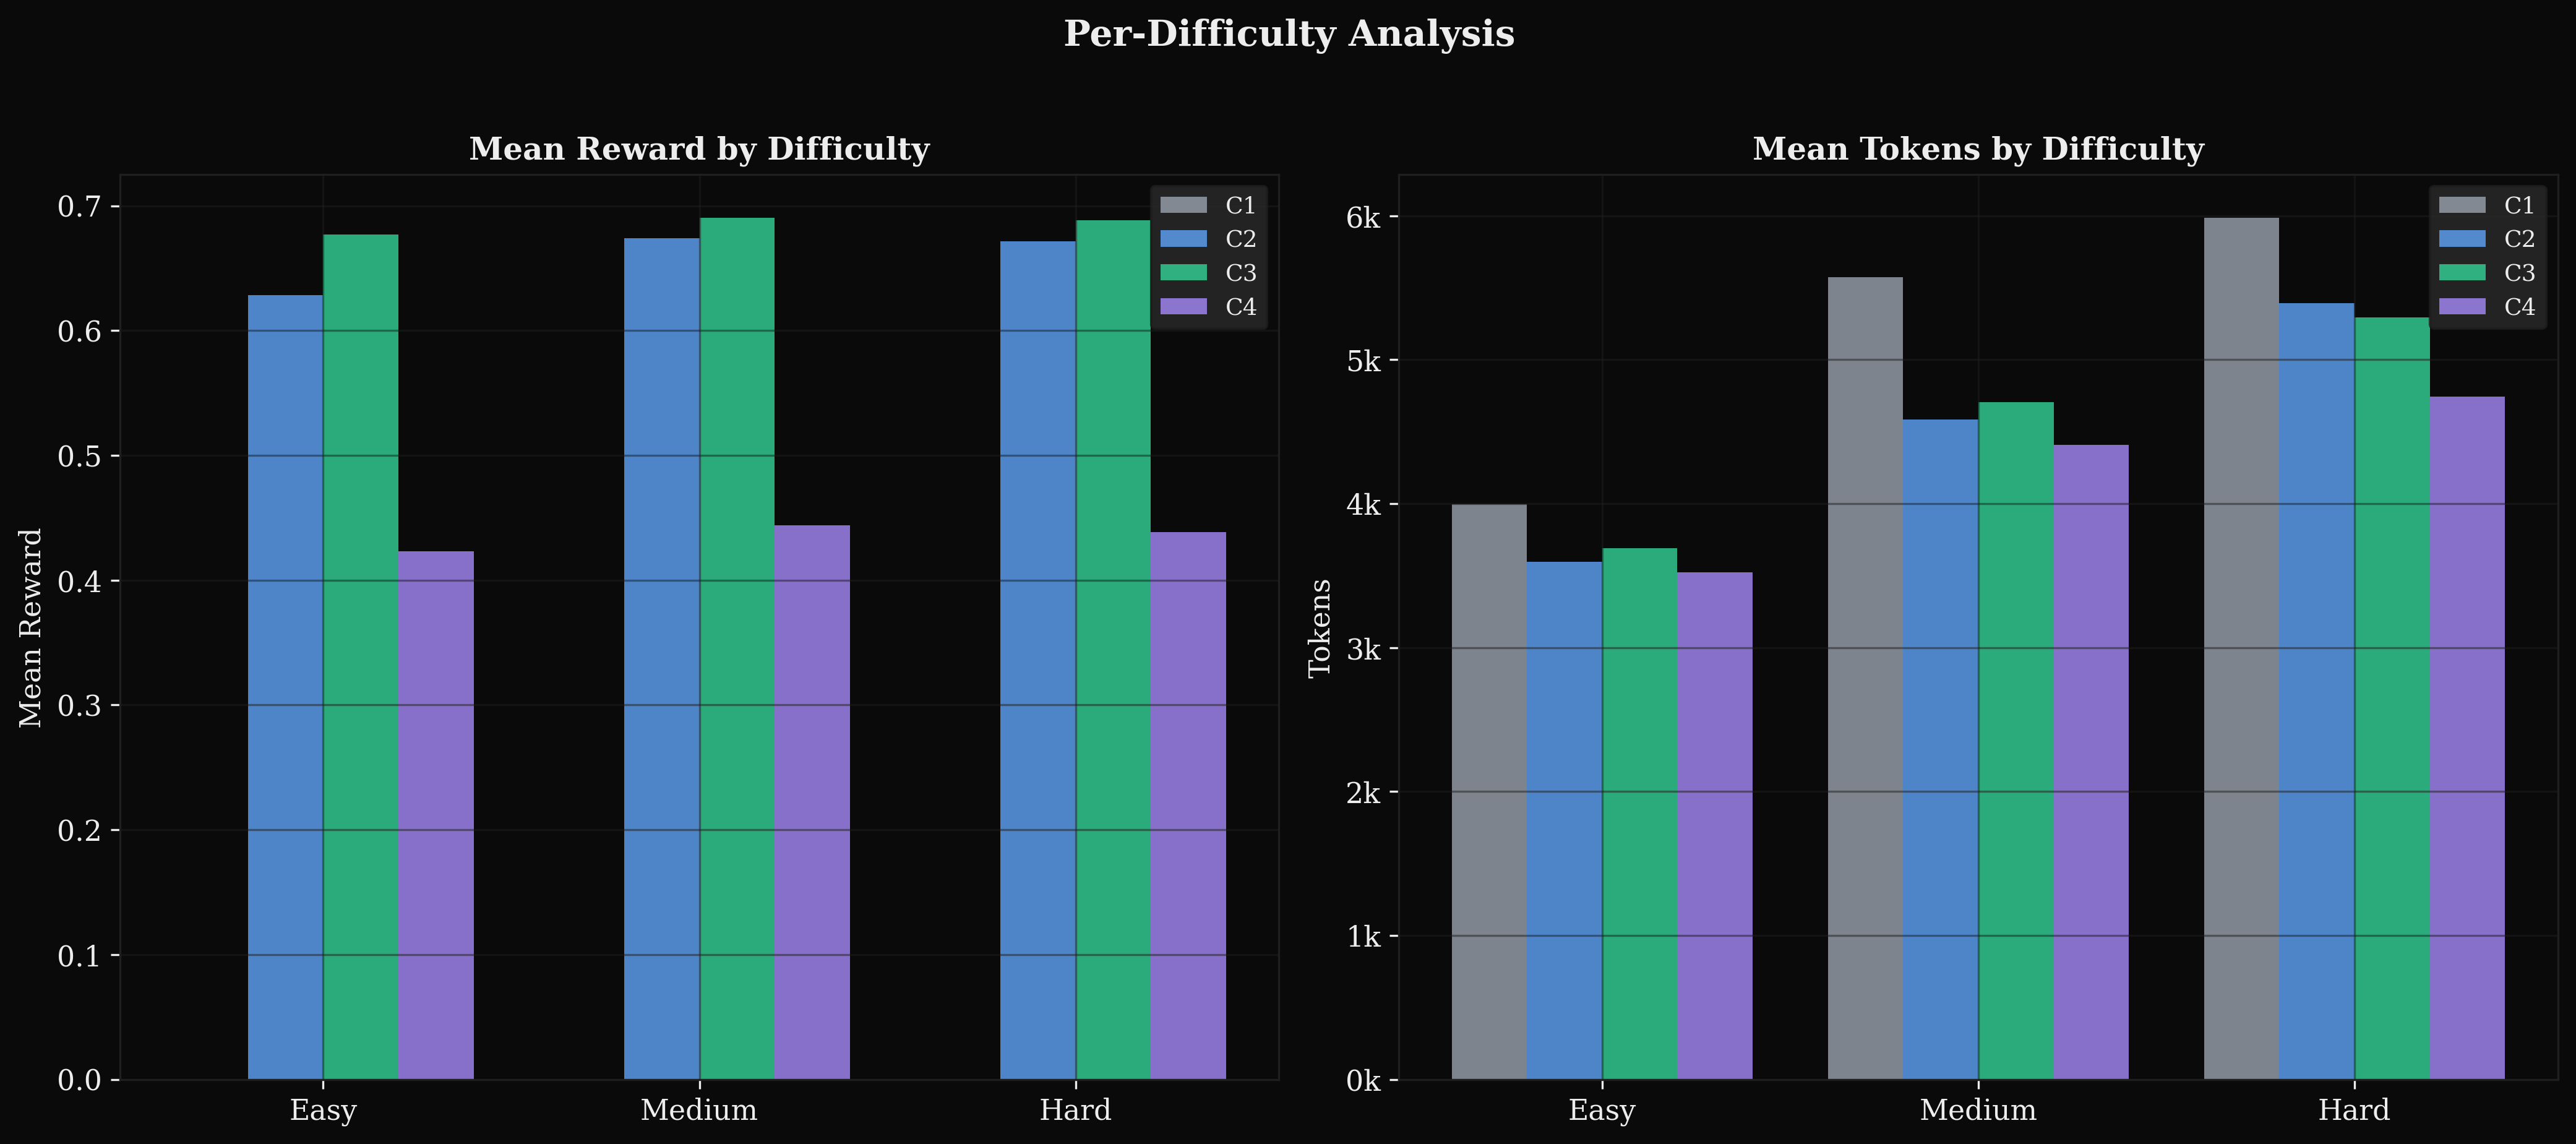
\includegraphics[width=\columnwidth]{../results/figures/figA8_difficulty_comparison.png}
\caption{Mean token consumption by difficulty level and condition (v3). The treatment effect scales with difficulty: $-$12\% for easy, $-$21\% for medium and hard tasks. Unlike Experiment~1 (where easy tasks showed rubric overhead), all difficulty levels benefit from the treatment in Experiment~2.}
\label{fig:v3_difficulty}
\end{figure}

\paragraph{Per-theme breakdown.}
The treatment effect varies across themes.
The largest reductions appear in retrieval\_systems (C1${=}$6{,}385, C4${=}$4{,}583, $-$28\%) and ml\_fundamentals (C1${=}$5{,}011, C4${=}$3{,}877, $-$23\%).
Themes where C1 generates the longest outputs benefit most from the rubric's output-constraining effect.
The smallest reduction is in evaluation\_methods (C1${=}$5{,}274, C4${=}$4{,}650, $-$12\%), possibly because evaluation tasks naturally produce more structured, concise responses even without rubric guidance (Figure~\ref{fig:v3_domain_heatmap}).

\begin{figure}[t]
\centering
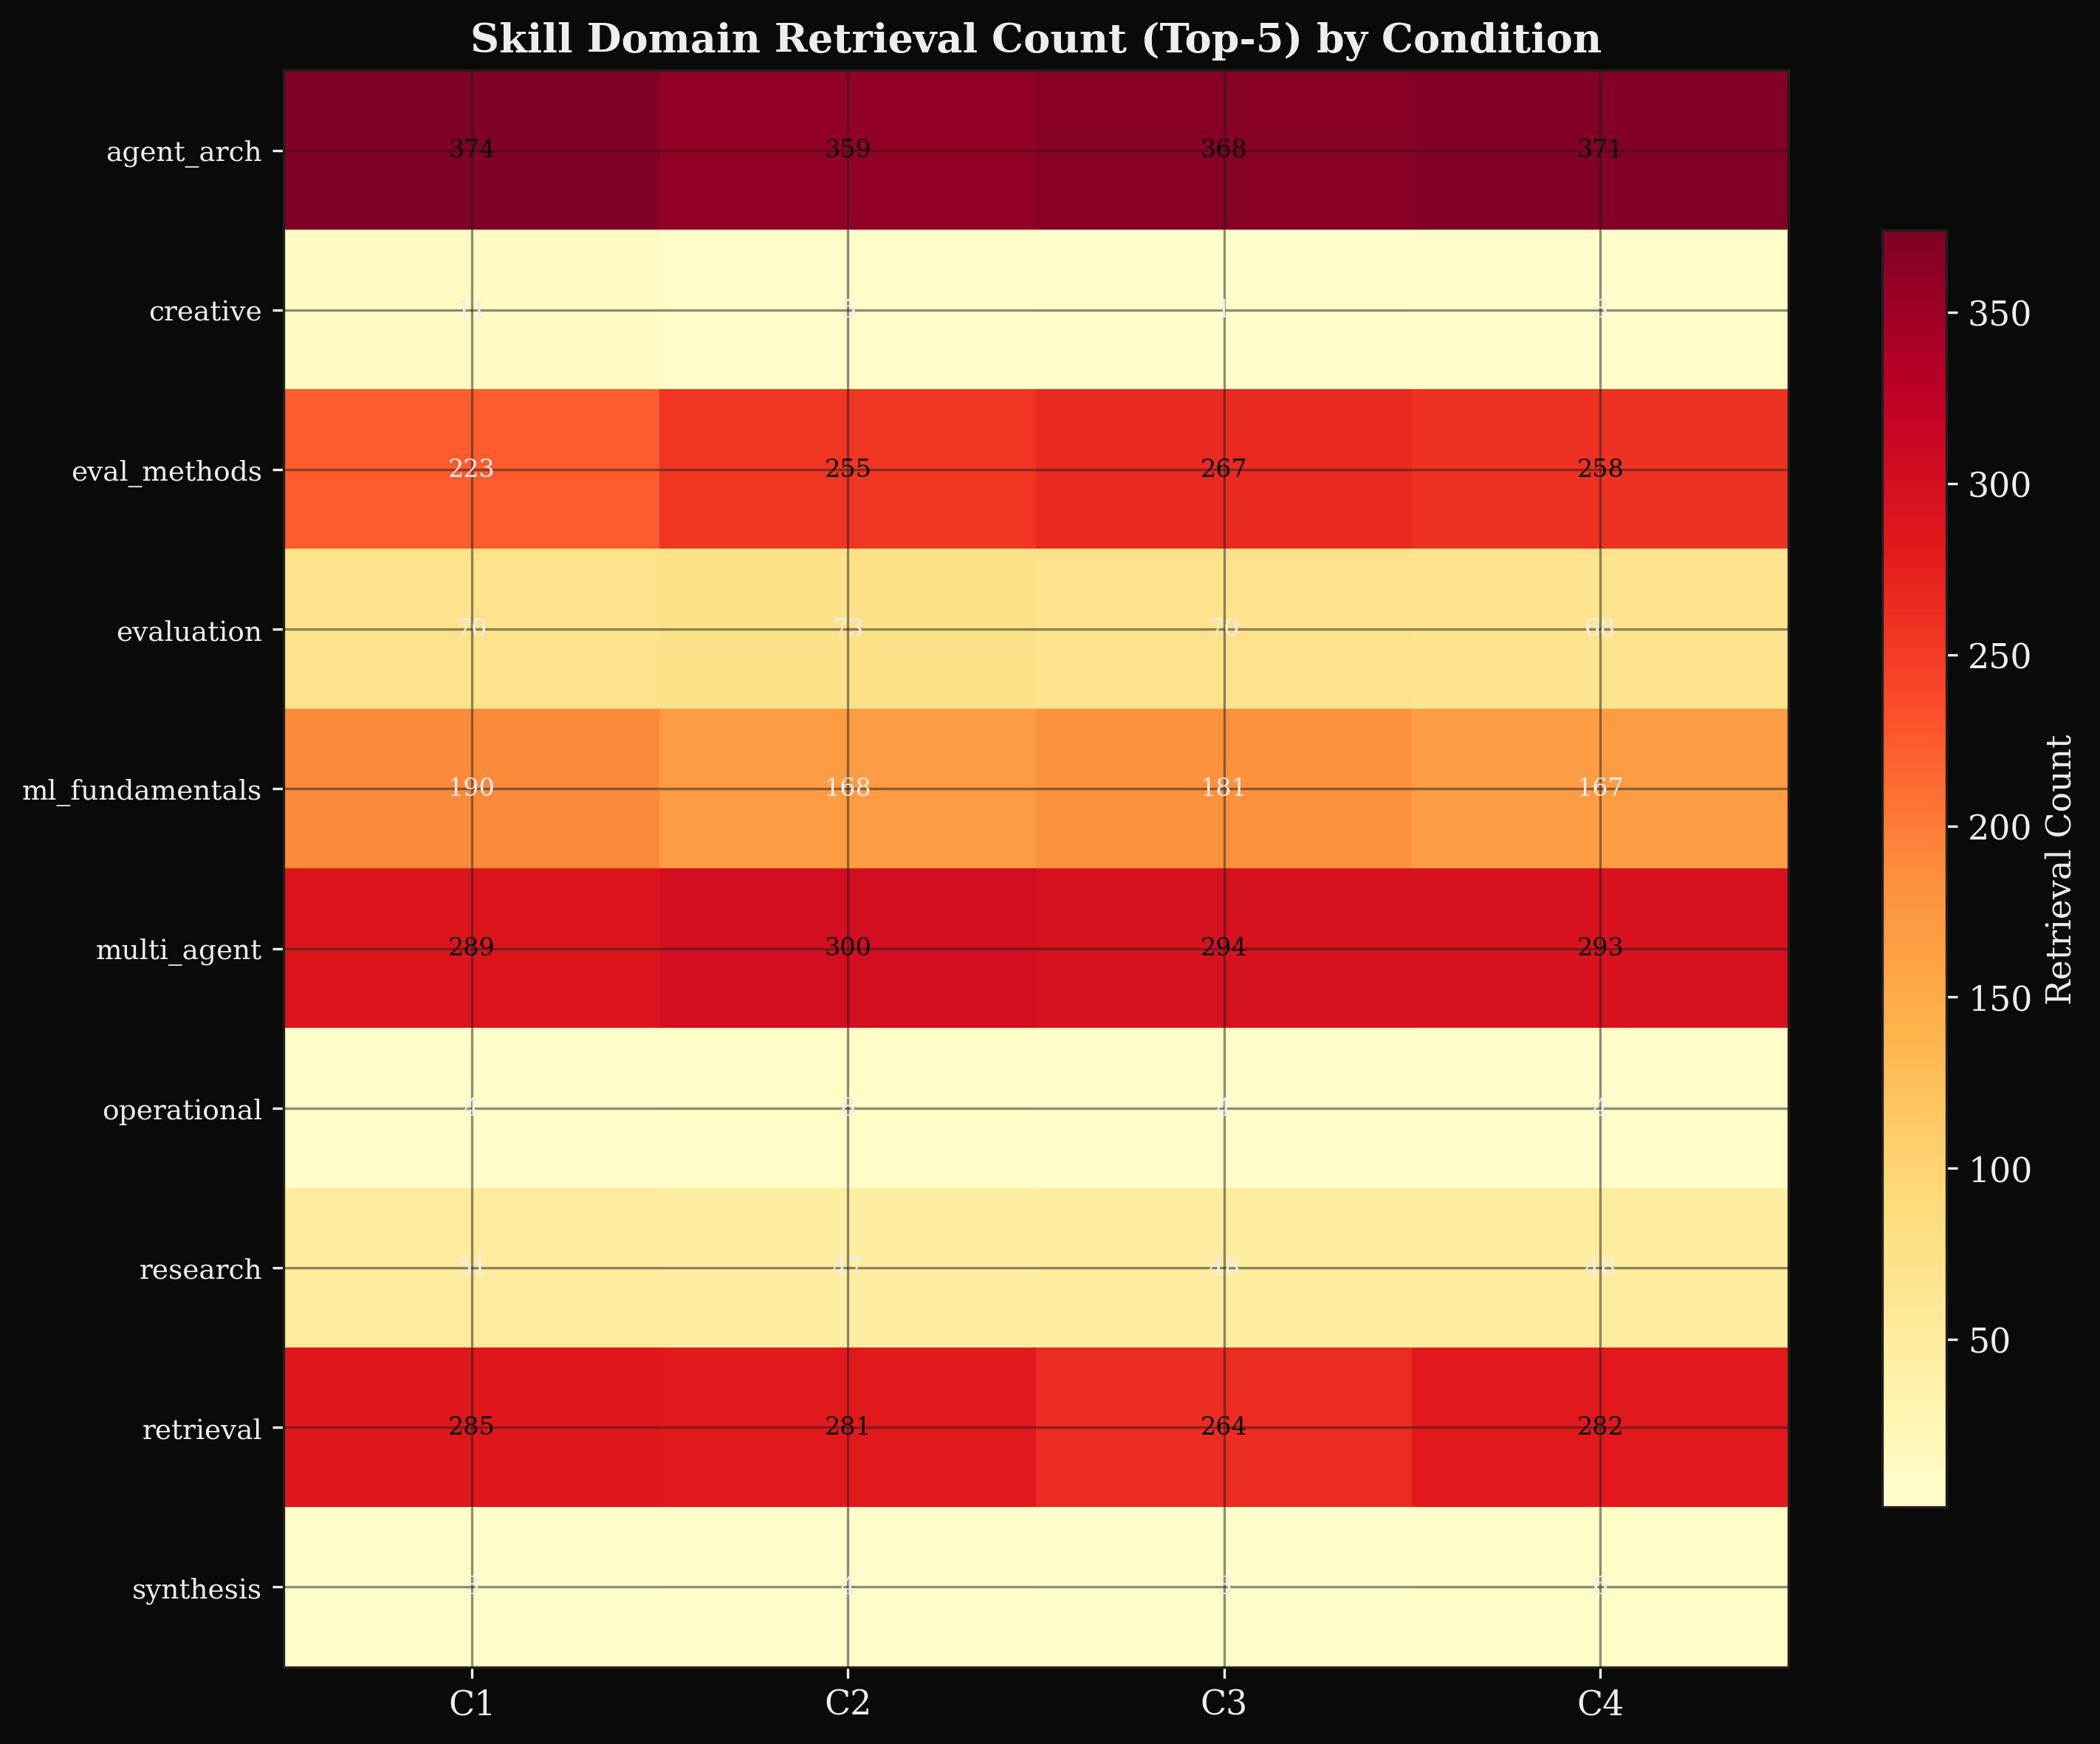
\includegraphics[width=\columnwidth]{../results/figures/figA9_domain_heatmap.png}
\caption{Mean token consumption by theme and condition (v3). Themes with the longest C1 outputs (retrieval\_systems, ml\_fundamentals) show the largest treatment effects, consistent with the output-driven mechanism: the rubric is most effective at reducing verbosity where verbosity is highest.}
\label{fig:v3_domain_heatmap}
\end{figure}

\paragraph{Two effects, now separable.}
Experiment~2 resolves the confound that limited Experiment~1's conclusions.
In v2, weight learning changed scores but not rankings (Jaccard $>$ 0.90), making it impossible to determine whether adaptive retrieval could contribute beyond the rubric prompt effect.
In v3, weight learning produces meaningfully different retrievals (mean Jaccard $<$ 0.60), with C3 achieving 26\% higher NDCG@5 than C1 and 20\% higher than C4.
Yet C4 achieves the largest token reduction ($-$19.7\% vs.\ C1), suggesting that \emph{the rubric prompt effect is the dominant mechanism for token reduction, while adaptive retrieval improves retrieval quality as measured by ground truth metrics}.

The two effects appear largely independent.
The rubric prompt effect reduces output token generation, a behavioral change in the LLM that does not depend on which skills were retrieved.
The adaptive retrieval effect improves the quality of retrieved skills, a change in the retrieval system that does not directly reduce token consumption when the rubric already constrains output verbosity.
This decomposition explains why C4 achieves the best efficiency (lowest mean tokens at 4{,}429, lowest output tokens at 2{,}537) while C3 achieves the best retrieval quality (highest NDCG@5 at 0.469, highest MRR at 0.411).

% Outlier Robustness Analysis — for inclusion in Section 5
% v3 re-run data (n=1200, 300 per condition, max_tokens=16384)

\subsection{Robustness to Outliers}
\label{sec:outlier_robustness}

With truncation cascades eliminated (\texttt{max\_tokens}$=$16{,}384), all four conditions produce relatively well-behaved distributions.
Mean-to-median ratios range from 1.08 (C4) to 1.15 (C2), with no extreme runaway episodes.
The single multi-step episode (C1, task~023, 21{,}259 tokens) is a moderate outlier at $6.4\sigma$ from the C1 mean.

To verify that the efficiency gains are not driven by a few high-token episodes, we apply progressively aggressive outlier filters, removing episodes exceeding $\mu + k\sigma$ for each condition independently at $k \in \{1, 2, 3\}$ (Table~\ref{tab:outlier_robustness}).

\begin{table}[t]
\centering
\small
\begin{tabular}{lccccc}
\toprule
\textbf{Filter} & \textbf{C1 mean} & \textbf{C2 mean} & \textbf{C3 mean} & \textbf{C4 mean} & \textbf{Best $\Delta$C1} \\
\midrule
None       & 5{,}517 & 4{,}824 & 4{,}830 & 4{,}429 & $-$19.7\% \\
$+3\sigma$ & 5{,}355 & 4{,}698 & 4{,}699 & 4{,}309 & $-$19.5\% \\
$+2\sigma$ & 5{,}190 & 4{,}533 & 4{,}555 & 4{,}224 & $-$18.6\% \\
$+1\sigma$ & 4{,}732 & 4{,}193 & 4{,}181 & 3{,}998 & $-$15.5\% \\
\bottomrule
\end{tabular}
\caption{Outlier robustness analysis. Each row removes episodes exceeding $\mu + k\sigma$ \emph{within each condition independently}. The treatment effect is stable across cutoffs (15--20\% reduction), confirming that the output-driven efficiency gain is distributed across the full episode population rather than driven by a few extreme episodes. ``Best $\Delta$C1'' reports the largest reduction among C2--C4 at each cutoff.}
\label{tab:outlier_robustness}
\end{table}

Two observations emerge.
First, the treatment effect is robust: even at the most aggressive filter ($+1\sigma$, which removes 39--48 episodes per condition), C4 still reduces mean tokens by 15.5\% relative to C1.
The stability across cutoffs (19.7\% raw $\rightarrow$ 15.5\% at $+1\sigma$) confirms that the effect is distributed across the full population of episodes, not concentrated in a few prevented catastrophes.
Second, unlike Experiment~1 where C1's mean was dominated by a catastrophic tail (mean/median ratio of 2.1$\times$), Experiment~2's clean distributions (all ratios $<$1.15) indicate that the output-driven mechanism operates consistently across all episodes.


\subsection{The Rubric Prompt Effect}
\label{sec:confound}

Experiment~1 revealed that C4 achieves the best token efficiency despite weak bandit convergence, suggesting a dominant prompt engineering effect.
Experiment~2 confirms and clarifies this finding in a more controlled setting: with truncation cascades eliminated, the rubric effect manifests as output compression rather than multi-step prevention.
C4 reduces mean tokens by 19.7\% while showing only weak bandit convergence (max posterior mean${=}$0.472), modest retrieval quality improvement (NDCG@5${=}$0.374 vs.\ C3's 0.469), and the lowest output token count (2{,}537 per episode).

The rubric prompt effect functions as a metacognitive anchor: by requiring the LLM to evaluate retrieval quality, regardless of whether that evaluation is used for adaptation, the rubric structures the response in a way that reduces verbose, exploratory output.
This has a methodological implication: \emph{any future work on adaptive retrieval in RAG systems must include a rubric-only control condition to isolate retrieval adaptation effects from prompt structuring effects.}

The contribution of weight learning is real but largely independent: C3 achieves substantially better retrieval (NDCG@5${=}$0.469 vs.\ C4's 0.374, $+$25\%) without improving token efficiency over C4.
This suggests that retrieval quality and token efficiency are partially independent outcomes in this setting, with the rubric's output-constraining effect introducing a ceiling: once the rubric has compressed output length, further retrieval quality improvements have limited room to produce additional token savings.
Improving retrieval quality through weight learning is valuable in its own right, ensuring the LLM receives the most relevant context, but the efficiency gains from the rubric's output-constraining effect are available without any learning at all.
